\documentclass[conference]{IEEEtran}
\IEEEoverridecommandlockouts
\usepackage[T1]{fontenc}
\usepackage{balance}
\usepackage{amsmath,amssymb}
\usepackage{graphicx,booktabs,array,tabularx,cite}
\usepackage[hidelinks]{hyperref}
\newcolumntype{Y}{>{\raggedright\arraybackslash}X}
\newcommand{\ket}[1]{\lvert #1\rangle}
\title{Quantum Algorithms versus Classical Algorithms:\\A Comparative Review and Ideal Search Study}
\author{\IEEEauthorblockN{SETTI APPALANAIDU\IEEEauthorrefmark{1}}
\IEEEauthorblockA{Department of CSE (AI \& ML)\\Marwadi University\\Rajkot, Gujarat, India\\\scriptsize\texttt{setti.139984@marwadiuniversity.ac.in}}
\and
\IEEEauthorblockN{Mohitrajsinh Jadeja}
\IEEEauthorblockA{Department of CSE (AI \& ML)\\Marwadi University\\Rajkot, Gujarat, India\\\scriptsize\texttt{mohitrajsinh.jadeja139200@marwadiuniversity.ac.in}}}
\begin{document}
\maketitle
\begingroup\renewcommand\thefootnote{\fnsymbol{footnote}}\footnotetext[1]{Corresponding author: SETTI APPALANAIDU.}\endgroup
\begin{abstract}
Quantum algorithms can reduce computational costs for selected tasks, but a complexity advantage does not by itself establish practical superiority over classical computation. This paper presents a focused comparative review of unstructured search, integer factorization, linear systems, quantum simulation, and variational optimization. Comparisons distinguish query complexity, logical operations, input access, output requirements, and physical implementation costs. A reproducible ideal state-vector study of Grover search covers search spaces from 16 to 65,536 candidates and checks simulated success probabilities against the analytical expression. At the largest size, 201 Grover iterations achieve a success probability of approximately 0.999988, compared with 32,768.5 expected checks for sequential classical search under a uniform target assumption. These are model-level resource counts, not measured hardware speedups. A simple sensitivity model illustrates how verification, repetition, and operation costs affect the crossover. The review concludes that meaningful quantum advantage requires a matched task, justified assumptions, a competitive classical baseline, and accounting for the complete computational workflow.
\end{abstract}
\begin{IEEEkeywords}
quantum algorithms, classical algorithms, computational complexity, Grover search, quantum advantage, comparative review
\end{IEEEkeywords}

\section{Introduction}
An algorithm specifies how a computational task is performed. Its efficiency depends on the task definition, input representation, output requirement, and available operations. Classical and quantum approaches should therefore be compared within a common problem specification rather than by treating one computing model as universally faster.

Quantum algorithm research includes search, number theory, simulation, and linear algebra. Montanaro provides a broad account of these algorithm families and their applications~\cite{montanaro}. Shor's factoring method and Grover's search method illustrate substantially different kinds of improvement~\cite{shor,grover}. The former exploits algebraic structure; the latter improves a black-box search task. Neither supports a general claim that a quantum computer solves every difficult problem efficiently.

This paper asks: \emph{Under which assumptions do selected quantum algorithms outperform their classical alternatives, and which costs can prevent a theoretical improvement from becoming a practical advantage?} The approach combines a focused literature review with a small, reproducible numerical case study. Its contribution is an educational synthesis and transparent resource-accounting example. It does not introduce a new quantum algorithm, prove a new complexity separation, or demonstrate hardware advantage.

The discussion separates three statements: a reduction in oracle queries, a reduction in logical operations under specified access assumptions, and a reduction in end-to-end physical execution cost. R\o nnow \emph{et al.} explain why definitions and baselines matter when evaluating quantum speedup~\cite{ronnow}. This distinction guides both the review and the numerical analysis.

\section{Computational Background}
\subsection{Classical and Quantum Representations}
Classical computation stores information as bits and supports deterministic, randomized, sequential, and parallel algorithms. Randomness and parallelism are therefore not exclusive features of quantum computing. Classical algorithms also exploit structure through indexing, sparsity, approximation, and problem-specific heuristics.

A pure state of $n$ qubits is represented as
\begin{equation}
\ket{\psi}=\sum_{x=0}^{2^n-1}\alpha_x\ket{x},\qquad
\sum_x |\alpha_x|^2=1.
\end{equation}
Quantum gates transform amplitudes, while measurement returns classical outcomes with probabilities determined by those amplitudes. Interference allows useful outcomes to be amplified. The existence of $2^n$ amplitudes does not provide direct access to $2^n$ classical answers. Reading an entire output vector may require extensive repetition, an issue especially relevant to quantum linear algebra~\cite{hhl,aaronson}.

\subsection{Complexity and Resource Measures}
Let $N$ denote the number of search candidates or a matrix dimension, and let $b$ denote the bit length of an integer. Polynomial complexity in $b$ differs from polynomial complexity in the integer value. Likewise, $O(\log N)$ dependence on matrix dimension can conceal significant dependence on conditioning, precision, or input preparation.

We distinguish oracle queries, gate counts, circuit depth, memory, and total execution cost. An oracle is an assumed interface for evaluating a function or accessing data. Assigning unit cost to an oracle is useful for proving a query bound, but implementing it may require a substantial circuit. Fault-tolerant implementations additionally distinguish logical qubits from physical qubits~\cite{fowler}. These measures cannot be substituted for one another without an explicit cost model.

\section{Review Scope and Comparison Method}
\subsection{Source Selection}
This is a focused narrative review, not an exhaustive systematic review or meta-analysis. Twenty scholarly references were selected to cover foundational algorithms, implementation costs, and challenges to advantage claims. The cited works span 1996--2021 publication or preprint dates; they are a deliberately bounded foundation rather than a survey of all developments through 2026.

Sources were located through title-based searches, publisher records, and arXiv records on 21 October 2026. Selection favored original algorithm papers for formal claims, with review articles for broader context. Relevant titles concerned search, factoring, linear systems, Hamiltonian simulation, variational methods, classical alternatives, and error correction. Popular summaries and product announcements were excluded from the manuscript bibliography. No database-wide screening count or comprehensive coverage is claimed.

\subsection{Extraction and Assessment}
For each family, the comparison records (i) the precise task, (ii) a suitable classical baseline, (iii) the claimed quantum improvement, (iv) input and output assumptions, and (v) costs omitted by the simplified bound. Where a general speedup is not established by the cited work, the paper states that limitation instead of assigning an unsupported complexity advantage.

Evidence is classified as a formal algorithmic result, a conditional resource estimate, a heuristic proposal, or a numerical illustration. The Grover case study is the last category. It verifies an established formula under ideal assumptions and is not evidence of new asymptotic behavior. Table~\ref{tab:comparison} summarizes the review; the following sections explain its qualifications.

\begin{table*}[t]
\caption{Task-matched comparison of selected algorithm families. Complexity statements use different models and are not direct wall-clock comparisons.}
\label{tab:comparison}
\centering\footnotesize
\setlength{\tabcolsep}{5pt}
\begin{tabularx}{\textwidth}{p{2.0cm}YYY}
\toprule
Task & Classical reference & Quantum result or approach & Conditions and interpretation\\
\midrule
Unstructured search & $\Theta(N)$ queries for constant success with one marked item & $\Theta(\sqrt N)$ queries using Grover search~\cite{grover,zalka} & Same black-box task; coherent oracle access; excludes oracle construction and physical gate costs.\\
Integer factorization & General number field sieve: heuristic subexponential time in bit length & Shor: polynomial-time quantum factoring~\cite{shor} & Relative to known classical methods; fault-tolerant arithmetic costs matter; no classical impossibility proof.\\
Linear-system features & Sparse iterative numerical methods; baseline depends on data access and required output & HHL prepares a solution-related quantum state with favorable dimension dependence~\cite{hhl} & Efficient state preparation, sparsity, conditioning, precision, and limited readout are essential.\\
Quantum dynamics & Exact state-vector evolution; structured approximations when applicable & Efficient simulation of suitable local or sparse Hamiltonians~\cite{lloyd,berry} & Hamiltonian description, evolution time, precision, and observable extraction must be specified.\\
Combinatorial optimization & Exact solvers, approximation algorithms, and tuned heuristics & QAOA combines parameterized circuits and classical optimization~\cite{farhi} & Instance- and depth-dependent; no blanket practical speedup follows from the proposal.\\
\bottomrule
\end{tabularx}
\end{table*}

\section{Comparative Analysis}
\subsection{Unstructured Search}
Consider a Boolean oracle $f$ with one marked input among $N$ candidates. Grover search alternates phase marking and a reflection about the initial uniform state~\cite{grover}. Boyer \emph{et al.} analyze the success probability and extensions to multiple or unknown solutions~\cite{boyer}. Zalka establishes optimality in the relevant black-box setting~\cite{zalka}.

The classical comparison is unstructured search, not binary search on an already sorted array. The latter uses a different information structure. Database indexing can similarly change the practical task, and its construction cost should be included when relevant. A query improvement is most informative when candidate evaluation can be implemented coherently at acceptable cost.

Amplitude amplification generalizes the search mechanism: a procedure with success probability $a$ can, under appropriate coherent access conditions, be amplified using a number of applications proportional to $1/\sqrt a$, instead of $1/a$ independent attempts~\cite{brassard}. This is a useful algorithmic primitive, but its access assumptions remain part of the result.

\subsection{Integer Factorization}
For a composite integer $M$ of bit length $b$, Shor's algorithm reduces factoring to an order-finding problem. Quantum period information is combined with classical number-theoretic processing. Its operation count is polynomial in $b$~\cite{shor}.

For comparison, the general number field sieve has heuristic running time of the form~\cite{pomerance}
\begin{equation}
\exp\!\left[\left((64/9)^{1/3}+o(1)\right)
(\ln M)^{1/3}(\ln\ln M)^{2/3}\right].
\end{equation}
This is subexponential in bit length rather than polynomial. Thus the comparison is a superpolynomial improvement over known classical methods, not a proof that every classical factoring algorithm must be slow~\cite{shor}.

Physical resource estimates tell a different part of the story. Gidney and Eker\aa{} translate a factoring construction into assumptions about error rates, code cycles, connectivity, repeated attempts, and layout~\cite{gidney}. Their estimate is an illustrative engineering study, not a measured cryptographic break or an assertion of the best available resource estimate in 2026. Practical feasibility cannot be inferred solely from a polynomial bound.

\subsection{Linear Systems and Data Access}
The HHL algorithm addresses features associated with a solution to $A x=b$, producing a normalized solution-related quantum state rather than printing every component of $x$~\cite{hhl}. Favorable dependence on matrix dimension requires suitable assumptions about access to $A$, preparation of $\ket b$, sparsity, condition number, and accuracy.

Comparing that output with a classical algorithm required to return the entire vector would mismatch the tasks. Aaronson emphasizes the input, conditioning, and readout qualifications behind attractive quantum machine-learning claims~\cite{aaronson}. For a proposed application, the relevant question is whether a useful statistic can be extracted economically, not simply whether a quantum state exists.

Classical baselines can also improve. Tang's recommendation-system algorithm shows that strong sampling-access assumptions can enable a classical alternative to a proposed exponential quantum advantage~\cite{tang}. This result concerns a particular recommendation setting; it does not eliminate every possible quantum machine-learning advantage. It demonstrates why equivalent data-access assumptions must be considered on both sides.

\subsection{Quantum Simulation}
Lloyd establishes efficient quantum simulation for suitable systems with local interactions~\cite{lloyd}. Berry \emph{et al.} improve the precision dependence of sparse-Hamiltonian simulation~\cite{berry}. These results concern specified dynamics and access models, not every problem involving chemistry or physics.

Exact classical state vectors have exponentially many amplitudes, but structured systems may admit effective classical approximations. Comparisons must therefore specify the Hamiltonian, desired evolution time, error tolerance, and observables. McArdle \emph{et al.} review quantum chemistry methods and the resource considerations needed to connect quantum computation with chemical questions~\cite{mcardle}. Preparing suitable states and extracting scientifically useful observables remain part of the total task.

\subsection{Variational Optimization}
QAOA uses alternating parameterized operations and a classical optimization process to seek approximate solutions~\cite{farhi}. The algorithm's existence does not establish that it outperforms the best classical solvers across arbitrary instances. Comparisons require matched solution quality, instance families, optimization budgets, and success criteria.

Cerezo \emph{et al.} discuss trainability, accuracy, and efficiency challenges in variational algorithms~\cite{cerezo}. McClean \emph{et al.} show that broad classes of parameterized circuits can exhibit gradients that become difficult to resolve as system size grows~\cite{mcclean}. These results should not be interpreted as a theorem that all variational circuits fail. They motivate careful ansatz design and explicit reporting of optimization and sampling costs.

\section{Reproducible Ideal Search Case Study}
\subsection{Model and Implementation}
The numerical study uses a real-valued state-vector simulator implemented with Python and NumPy. Each search space has $N=2^n$ candidates, $n\in\{4,\ldots,16\}$, with one marked target at index zero. The initial amplitudes are $1/\sqrt N$. One iteration negates the marked amplitude and then applies inversion about the mean to every amplitude. No noise, routing constraints, gate decomposition, measurement sampling, or physical quantum processor is modeled.

For one target, define
\begin{equation}
\theta=\arcsin(1/\sqrt N),\qquad
P_k=\sin^2((2k+1)\theta).
\label{eq:prob}
\end{equation}
This established success formula~\cite{boyer} is evaluated independently of the state-vector updates. The integer iteration choice is
\begin{equation}
k_\star=\left\lfloor\frac{\pi}{4\theta}\right\rfloor,
\end{equation}
which selects a nearest integer to the first continuous probability maximum, with either choice admissible in a tie.

The simulation checks probability agreement and state normalization to an absolute tolerance of $10^{-10}$. Because this calculation propagates an ideal state rather than sampling shots, the reported probabilities are deterministic numerical values. There are no statistical confidence intervals to estimate. The supplementary source regenerates both figures and the complete 13-row results table.

\subsection{Classical Baseline and Fairness}
For sequential search without replacement and a uniformly located target, the number of checks is uniformly distributed over $1,\ldots,N$. Therefore
\begin{equation}
E[C]=\frac{1}{N}\sum_{j=1}^{N}j=\frac{N+1}{2}.
\label{eq:classical}
\end{equation}
The fixed quantum target position does not change its ideal success probability because all initial amplitudes are identical. The classical expectation corresponds to averaging target positions, or equivalently randomizing the order of checking a fixed target. It must not be interpreted as the cost of a deterministic scan that starts at the known marked index.

Figure~\ref{fig:scaling} compares this classical expected count with the quantum iteration count. A single Grover attempt can fail, whereas the classical scan eventually succeeds. Consequently, that plot illustrates resource scaling and is not by itself a matched time-to-solution comparison. Verification and repetition are included separately below.

\begin{figure}[t]
\centering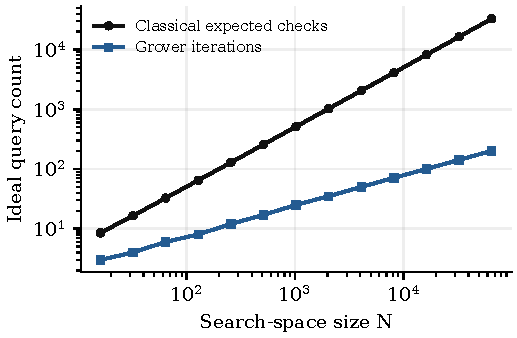
\includegraphics[width=\columnwidth]{query_scaling.pdf}
\caption{Ideal search resource counts from the reproducible case study. Classical counts are expectations over a uniform target; quantum counts describe one attempt before final verification. Axes are logarithmic. No execution-time measurements are shown.}
\label{fig:scaling}
\end{figure}

\subsection{Numerical Results}
Table~\ref{tab:results} reports four representative sizes; the CSV includes all sizes. The simulated probability agrees with~\eqref{eq:prob} within the stated tolerance. For $N=65,536$, 201 iterations yield $P_{201}\approx0.99998826$. The corresponding classical expectation is $32,768.5$ checks. The raw count ratio is approximately $163.03$, before accounting for final verification or unsuccessful attempts.

\begin{table}[t]
\caption{Selected ideal simulation results. $E[C]$ is the classical expectation; $k_\star$ is the number of Grover iterations.}
\label{tab:results}
\centering\footnotesize
\begin{tabular}{rrrrr}
\toprule
$N$ & $k_\star$ & $P_{k_\star}$ & $E[C]$ & $E[C]/k_\star$\\
\midrule
16 & 3 & 0.961319 & 8.5 & 2.83\\
256 & 12 & 0.999947 & 128.5 & 10.71\\
4,096 & 50 & 0.999945 & 2,048.5 & 40.97\\
65,536 & 201 & 0.999988 & 32,768.5 & 163.03\\
\bottomrule
\end{tabular}
\end{table}

Figure~\ref{fig:probability} shows why the iteration count matters. Success increases toward the first maximum and then decreases because amplitude amplification rotates past the target direction. More iterations do not monotonically increase success. The simulator reproduces this oscillation for $N=256$.

\begin{figure}[t]
\centering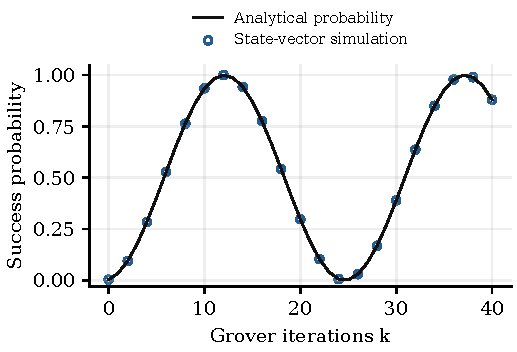
\includegraphics[width=\columnwidth]{success_probability.pdf}
\caption{Success probability for one marked item among 256 candidates. The line is the analytical expression; markers are independently propagated state-vector values at every second iteration.}
\label{fig:probability}
\end{figure}

\subsection{Sensitivity to Verification and Operation Cost}
To expose omitted costs, consider a deliberately simplified accounting model. Assign cost $c$ to a classical predicate check. Let $r c$ be the cost of a complete Grover iteration, including its oracle and diffusion, and conservatively assign the same cost to final verification. Let $H\geq0$ include preparation and other overhead per attempt, and set $h=H/c$. Independent attempts are repeated after failed verification, with success probability $P=P_{k_\star}$. The expected normalized quantum cost is then
\begin{equation}
E[T_Q]/c=\frac{h+r(k_\star+1)}{P}.
\label{eq:cost}
\end{equation}
This is an illustrative model, not a fitted hardware estimate. The equal verification-cost assumption can be replaced when a specific implementation is available. From~\eqref{eq:classical} and~\eqref{eq:cost}, an expected-cost advantage requires
\begin{equation}
r<\frac{P(N+1)/2-h}{k_\star+1}.
\label{eq:crossover}
\end{equation}
For $N=65,536$ and $h=0$, the threshold is approximately $162.22$. Thus an assumed $r=200$ would remove the expected-cost advantage even though the raw query ratio is about 163. For $N=256$, the zero-overhead threshold is only about $9.88$. These examples show that a quadratic query improvement can coexist with poor practical performance. They do not predict an actual device crossover.

\section{Practical Implications and Limitations}
\subsection{From Logical Algorithms to Physical Workflows}
Preskill's discussion of noisy intermediate-scale computation emphasizes that limited circuit reliability constrains useful computations~\cite{preskill}. Surface-code methods illustrate the substantial engineering distinction between a logical operation and its physical realization~\cite{fowler}. Relevant accounting can include state preparation, error correction, compilation, communication, measurement, and classical processing. Which costs dominate depends on the application and architecture.

Our numerical simulator does not model those effects. It runs on a classical computer and explicitly stores all $N$ amplitudes. Each simulated diffusion step touches the whole vector, so simulator execution time is not the query cost of a physical quantum algorithm. The study verifies an ideal recurrence; it cannot demonstrate a quantum runtime advantage.

\subsection{Implications for Applications}
Factoring motivates examination of cryptographic assumptions, while simulation motivates chemistry and materials applications~\cite{shor,mcardle}. Search and amplification can support subroutines in broader workflows~\cite{brassard}. However, the costs and output requirements of the surrounding application must be included before extrapolating from a subroutine to a complete system.

For optimization and machine learning, a credible comparison should use tuned classical alternatives and equivalent preprocessing access. Tang's result illustrates how such access can change a baseline~\cite{tang}. Variational applications must also budget repeated measurements and classical parameter updates~\cite{cerezo}. A successful small example is insufficient to establish scalable superiority.

\subsection{Scope of the Conclusions}
The review uses a small purposive literature set and does not rank every known algorithm. It does not survey recent hardware milestones or establish which implementation is best in 2026. No energy, financial-cost, or wall-clock measurements were collected. The search study assumes one known-to-exist solution, ideal operations, and readily available coherent predicate access.

The crossover expression is an accounting illustration, not a new lower bound or an engineering forecast. Its assumptions intentionally remain explicit so a later hardware study can replace them. Further work could evaluate compiled oracle circuits, several target densities, noisy execution, and optimized classical parallel baselines under matched confidence and output criteria. Such work would require additional experiments beyond this manuscript.

\balance
\section{Conclusion}
Quantum and classical algorithms should be compared through matched computational tasks and explicit resource models. The reviewed literature supports a quadratic black-box search improvement, a polynomial-time quantum factoring method relative to known classical alternatives, and conditional opportunities in linear algebra and quantum simulation. Variational optimization requires case-specific evidence rather than a universal speedup claim.

The reproducible Grover study confirms the established ideal success expression across 13 search-space sizes and illustrates why oracle counts alone do not establish practical advantage. At 65,536 candidates, 201 iterations produce approximately 0.999988 success probability, but verification, repetition, and operation costs alter the comparison. The central implication is methodological: practical advantage requires useful outputs, justified access assumptions, competitive classical baselines, and complete workflow accounting.

\section*{Reproducibility and Research Scope}
The accompanying source package contains the simulator, numerical CSV, environment versions, and figure-generation code. No human-participant data or external experimental dataset is used. The study is a review with an ideal numerical illustration; all new numerical values are generated by the supplied code. No hardware benchmark, novel algorithm, or publication acceptance is claimed.

\begin{thebibliography}{20}
\bibitem{montanaro} A. Montanaro, ``Quantum algorithms: An overview,'' \emph{npj Quantum Information}, vol. 2, Art. no. 15023, 2016, doi: \href{https://doi.org/10.1038/npjqi.2015.23}{10.1038/npjqi.2015.23}.
\bibitem{shor} P. W. Shor, ``Polynomial-time algorithms for prime factorization and discrete logarithms on a quantum computer,'' \emph{SIAM Journal on Computing}, vol. 26, no. 5, pp. 1484--1509, 1997, doi: \href{https://doi.org/10.1137/S0097539795293172}{10.1137/S0097539795293172}.
\bibitem{grover} L. K. Grover, ``A fast quantum mechanical algorithm for database search,'' in \emph{Proc. 28th Annual ACM Symposium on Theory of Computing}, 1996, pp. 212--219. [Online]. Available: \url{https://arxiv.org/abs/quant-ph/9605043}
\bibitem{ronnow} T. F. R\o nnow \emph{et al.}, ``Defining and detecting quantum speedup,'' \emph{Science}, vol. 345, no. 6195, pp. 420--424, 2014, doi: \href{https://doi.org/10.1126/science.1252319}{10.1126/science.1252319}.
\bibitem{hhl} A. W. Harrow, A. Hassidim, and S. Lloyd, ``Quantum algorithm for linear systems of equations,'' \emph{Physical Review Letters}, vol. 103, Art. no. 150502, 2009, doi: \href{https://doi.org/10.1103/PhysRevLett.103.150502}{10.1103/PhysRevLett.103.150502}.
\bibitem{aaronson} S. Aaronson, ``Read the fine print,'' \emph{Nature Physics}, vol. 11, pp. 291--293, 2015, doi: \href{https://doi.org/10.1038/nphys3272}{10.1038/nphys3272}.
\bibitem{fowler} A. G. Fowler, M. Mariantoni, J. M. Martinis, and A. N. Cleland, ``Surface codes: Towards practical large-scale quantum computation,'' \emph{Physical Review A}, vol. 86, Art. no. 032324, 2012. [Online]. Available: \url{https://arxiv.org/abs/1208.0928}
\bibitem{zalka} C. Zalka, ``Grover's quantum searching algorithm is optimal,'' \emph{Physical Review A}, vol. 60, pp. 2746--2751, 1999, doi: \href{https://doi.org/10.1103/PhysRevA.60.2746}{10.1103/PhysRevA.60.2746}.
\bibitem{lloyd} S. Lloyd, ``Universal quantum simulators,'' \emph{Science}, vol. 273, no. 5278, pp. 1073--1078, 1996, doi: \href{https://doi.org/10.1126/science.273.5278.1073}{10.1126/science.273.5278.1073}.
\bibitem{berry} D. W. Berry, A. M. Childs, R. Cleve, R. Kothari, and R. D. Somma, ``Exponential improvement in precision for simulating sparse Hamiltonians,'' in \emph{Proc. 46th Annual ACM Symposium on Theory of Computing}, 2014, pp. 283--292, doi: \href{https://doi.org/10.1145/2591796.2591854}{10.1145/2591796.2591854}.
\bibitem{farhi} E. Farhi, J. Goldstone, and S. Gutmann, ``A quantum approximate optimization algorithm,'' arXiv:1411.4028, 2014. [Online]. Available: \url{https://arxiv.org/abs/1411.4028}
\bibitem{pomerance} C. Pomerance, ``A tale of two sieves,'' \emph{Notices of the American Mathematical Society}, vol. 43, no. 12, pp. 1473--1485, 1996. [Online]. Available: \url{https://www.ams.org/notices/199612/pomerance.pdf}
\bibitem{boyer} M. Boyer, G. Brassard, P. H\o yer, and A. Tapp, ``Tight bounds on quantum searching,'' \emph{Fortschritte der Physik}, vol. 46, pp. 493--505, 1998. [Online]. Available: \url{https://arxiv.org/abs/quant-ph/9605034}
\bibitem{brassard} G. Brassard, P. H\o yer, M. Mosca, and A. Tapp, ``Quantum amplitude amplification and estimation,'' arXiv:quant-ph/0005055, 2000. [Online]. Available: \url{https://arxiv.org/abs/quant-ph/0005055}
\bibitem{gidney} C. Gidney and M. Eker\aa{}, ``How to factor 2048 bit RSA integers in 8 hours using 20 million noisy qubits,'' \emph{Quantum}, vol. 5, Art. no. 433, 2021. [Online]. Available: \url{https://arxiv.org/abs/1905.09749}
\bibitem{tang} E. Tang, ``A quantum-inspired classical algorithm for recommendation systems,'' in \emph{Proc. 51st Annual ACM SIGACT Symposium on Theory of Computing}, 2019, pp. 217--228, doi: \href{https://doi.org/10.1145/3313276.3316310}{10.1145/3313276.3316310}.
\bibitem{mcardle} S. McArdle, S. Endo, A. Aspuru-Guzik, S. C. Benjamin, and X. Yuan, ``Quantum computational chemistry,'' \emph{Reviews of Modern Physics}, vol. 92, Art. no. 015003, 2020. [Online]. Available: \url{https://arxiv.org/abs/1808.10402}
\bibitem{cerezo} M. Cerezo \emph{et al.}, ``Variational quantum algorithms,'' \emph{Nature Reviews Physics}, vol. 3, pp. 625--644, 2021. [Online]. Available: \url{https://arxiv.org/abs/2012.09265}
\bibitem{mcclean} J. R. McClean, S. Boixo, V. N. Smelyanskiy, R. Babbush, and H. Neven, ``Barren plateaus in quantum neural network training landscapes,'' \emph{Nature Communications}, vol. 9, Art. no. 4812, 2018. [Online]. Available: \url{https://arxiv.org/abs/1803.11173}
\bibitem{preskill} J. Preskill, ``Quantum computing in the NISQ era and beyond,'' \emph{Quantum}, vol. 2, Art. no. 79, 2018. [Online]. Available: \url{https://arxiv.org/abs/1801.00862}
\end{thebibliography}
\end{document}
